% !TeX spellcheck = en_GB
% !TeX program = lualatex
%
% v 2.3  Feb 2019   Volker RW Schaa
%		# changes in the collaboration therefore updated file "jacow-collaboration.tex"
%		# all References with DOIs have their period/full stop before the DOI (after pp. or year)
%		# in the author/affiliation block all ZIP codes in square brackets removed as it was not %         understood as optional parameter and ZIP codes had bin put in brackets
%       # References to the current IPAC are changed to "IPAC'19, Melbourne, Australia"
%       # font for ‘url’ style changed to ‘newtxtt’ as it is easier to distinguish "O" and "0"
%
\documentclass[a4paper,
               %boxit,        % check whether paper is inside correct margins
               %titlepage,    % separate title page
               %refpage       % separate references
               biblatex,     % biblatex is used
               keeplastbox,   % flushend option: not to un-indent last line in References
               %nospread,     % flushend option: do not fill with whitespace to balance columns
               %hyphens,      % allow \url to hyphenate at "-" (hyphens)
               %xetex,        % use XeLaTeX to process the file
               %luatex,       % use LuaLaTeX to process the file
               ]{jacow}
%
% ONLY FOR \footnote in table/tabular
%
\usepackage{pdfpages,multirow,ragged2e} %
%
% CHANGE SEQUENCE OF GRAPHICS EXTENSION TO BE EMBEDDED
% ----------------------------------------------------
% test for XeTeX where the sequence is by default eps-> pdf, jpg, png, pdf, ...
%    and the JACoW template provides JACpic2v3.eps and JACpic2v3.jpg which
%    might generates errors, therefore PNG and JPG first
%
\makeatletter%
	\ifboolexpr{bool{xetex}}
	 {\renewcommand{\Gin@extensions}{.pdf,%
	                    .png,.jpg,.bmp,.pict,.tif,.psd,.mac,.sga,.tga,.gif,%
	                    .eps,.ps,%
	                    }}{}
\makeatother

% CHECK FOR XeTeX/LuaTeX BEFORE DEFINING AN INPUT ENCODING
% --------------------------------------------------------
%   utf8  is default for XeTeX/LuaTeX
%   utf8  in LaTeX only realises a small portion of codes
%
\ifboolexpr{bool{xetex} or bool{luatex}} % test for XeTeX/LuaTeX
 {}                                      % input encoding is utf8 by default
 {\usepackage[utf8]{inputenc}}           % switch to utf8

\usepackage[USenglish]{babel}

%
% if BibLaTeX is used
%
\addbibresource{FR1BCO03.bib}

%%
%%   Lengths for the spaces in the title
%%   \setlength\titleblockstartskip{..}  %before title, default 3pt
%%   \setlength\titleblockmiddleskip{..} %between title + author, default 1em
%%   \setlength\titleblockendskip{..}    %afterauthor, default 1em

\begin{document}

\title{SKA Project Status Update}

\author{N. P. Rees\thanks{Nick.Rees@skao.int}, SKA Observatory, Jodrell Bank, UK\\
		on behalf of the The SKA Software Collaboration\thanks{See Appendix}}
		}


\maketitle

%
\begin{abstract}
The SKA Project is a science mega-project whose mission is to build the world's two largest radio telescopes with sensitivity, angular resolution, and survey speed far surpassing current state-of-the-art instruments at relevant radio frequencies. The Low Frequency telescope, SKA-Low, is designed to observe between 50 and 350 MHz and will be built at Inyarrimanha Ilgari Bundara, the CSIRO Murchison Radio-astronomy Observatory in Western Australia. The Mid Frequency telescope, SKA-Mid, is designed to observe between 350 MHz and 15 GHz and will be built in the Meerkat National Park, in the Northern Cape of South Africa. Each telescope will be delivered in a number of stages, called Array Assemblies. Each Array Assembly will be a fully working telescope which will allow us to understand the design and potentially improve the system to deliver a better scientific instrument for the users. The final control system will consist of around 2 million control points per telescope, and the first Array Assembly, known as AA0.5, is being delivered at the time of ICALEPCS 2023.
\end{abstract}

\section{INTRODUCTION}
This is the third in a series of SKA status papers presented at ICALEPCS meetings and should be read in conjunction with the other two to understand the evolution of the SKA. At the time of the 2021 paper formal construction had just commenced in July of that year, and we were in the process of issuing the first round of contracts. This paper covers the evolution since this time, but it starts with a brief historical overview to establish context.

\section{HISTORY}
Although SKAO was officially created as an international observatory on 15 January 2021, the concept dates back to the early 1990's when astronomers proposed the idea of tracing the history of the Universe by mapping its most abundant element: Hydrogen (see, for example, Wilkinson~\cite{1991ASPC...19..428W}). Specifically, they proposed to observe the H1 emission line from it's rest frequency of 1420 MHz to red-shifts of more than 10, thereby observing it from the present day to just after the beginning of the universe.

To achieve this goal required a telescope of unparalleled sensitivity, with a collecting area approaching a square kilometre, and a frequency range from less than 100 MHz to a few GHz. Of course, once these basic parameters were described, scientists realised this basic instrument would be capable of observing a huge number of phenomena. Whilst this significantly enhanced the science case and scientific interest in the project, it also complicated the design, and necessitated the construction of two telescopes - one optimised for mid frequencies between 0.35 and 15 GHz and the other between 50 and 350 MHz.

The project has always been seen as international in scope, and in 2013 it was decided to establish an Inter-governmental Organisation to manage construction and operate the telescopes.

% \begin{itemize}[nosep,leftmargin=30pt]
% %% [itemsep=0pt]
%     \item[1988] Independent suggestions for a Large Radio Telescope
%     \item[1990] 10th anniversary of VLA – the visions merge
%     \item[1993] URSI GA Kyoto resolution to establish the Large Telescope Working Group 
%     \item[1994] IAU forms its Future Large Scale Facilities Working Group 
%     \item[1996] OECD Global Science Forum included radio astronomy activities
%     \item[1997] MoA for technology collaboration
%     \item[1998] “SKA” name adopted
%     \item[2000] International MoU signed
%     \item[2003] SKA International Project Office established in the Netherlands
%     \item[2004] Rawlings and Carilli published the new science case
%     \item[2006] Site down-selected to Australia and South Africa
%     \item[2008] SKA Project Development Office (SPDO) formed
%     \item[2009] Agencies SKA Group formed
%     \item[2011] SKA Organisation becomes a legal entity - a UK limited company.
%     \item[2012] Selection of the SKA host sites in Australia and South Africa
%     \item[2013] SKA Design Consortia commence design of telescope components
%     \item[2014] Rebaselining of the project into SKA1 and SKA2.
%     \item[2015] Jodrell Bank selected as the permanent home of the SKA Observatory
% \end{itemize}
% 1993 when a, international group of  astronomers began collaborating on developing world’s next-generation low-frequency telescope. The collaboration – known as SKA Telescope – was an informal affiliation. During these early years, there was neither a formal treaty to govern the relationship nor formal contracts. Rather, it was a group of pioneering, like-minded individuals and organizations all collaborating to unlock the art of the possible to show proof of concept for a large-scale radio telescope.


\subsection{Pre-Construction}
Prior to the formal start of construction the SKA had an extended pre-construction phase, culminated in a period of detailed design by pre-construction consortia from ~2014 to ~2018, followed by a bridging phase aftger the designs had passed CDR but the construction had no formally started. In software, this was far from ideal, because the design consortia did limited prototyping, and consequently limited practical design validation, so the value was limited because it was largely limited to a paper exercise. This changed in the bridging phase, where we pivoted to focussing on development of processes with the adoption of the Scaled Agile Framework, and code creation.

\subsection{Construction}
At the time of the last paper construction had only just commenced. The plan is to build the two telescopes simultaneously, and each is to be delivered in stages, as successfuly larger and more powerful interferometers. Each stage is known as an ''Array Assembly (AA)'', and the basic parameters of each array assembly is shown in table~\ref{tab:array-assemblies}. An outline of the major delivery milestones for both telescopes is shown in Figure~\ref{fig:ska-timeline}

\begin{table*}[!h]
	\centering
	\caption{Basic parameters for SKA major milestones. The Operations Readiness Review }
        \begin{tabular}{llcc}
            \toprule
            Milestone Event (earliest) & Array Size & SKA-Mid (end date) & SKA-Mid (end date)\\
            \midrule
            AA0.5 & 4 dishes 6 stations   & 2025 Jan & 2024 Nov\\
            AA1   & 8 dishes 18 stations  & 2026 Jan & 2025 Nov\\
            AA2   & 64 dishes 64 stations & 2027 Jan & 2026 Oct\\
            AA3 & 121 dishes 256 stations &  & \\
            AA* & 144 dishes 307 stations & 2027 Oct & 2028 Jan\\
            \multicolumn{2}{l}{Operations Readiness Review} & 2028 Jan & 2028 Apr\\
            \multicolumn{2}{l}{End of Staged Delivery programme} & 2028 Jul & 2028 Jul\\
            AA4 & 197 dishes 512 stations & TBD & TBD\\
            \bottomrule
        \end{tabular}
	\label{tab:array-assemblies}
 \end{table*}

 \begin{figure*}[tb]
	\centering
	  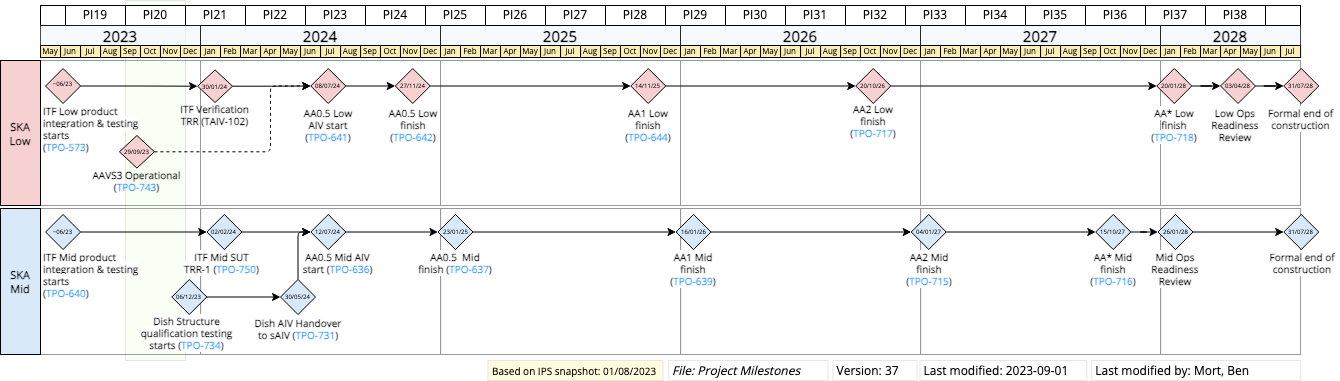
\includegraphics[width=\textwidth]{FR1BCO03f2.png}
	\caption{
		Graphical representation of the SKA project schedule as at 1 August 2023. Milestones dates do not include any allowance for schedule contingency, so the actual dates are anticipated to be delayed in a managed way.
	}
	\label{fig:ska-timeline}
  \end{figure*}

As of August 2023, 70 contracts and significant purchase orders have been awarded for a total commitment of approximately €575M. These contracts range across the major infrastructure works in each country as well as the technical subsystems and services required for complete facility systems, focusing on the long lead items needed for early deliveries but including full scale Staged Deliveries as well. Recently, for example, contracts were emndorsed for the main access, airstrip and site accommodation for the SKA-Low telescope in Australia, and delivery of 64 Dish Structure Systems for the SKA-Mid telescope in South Africa. was also signed, following on from last year’s signature of the In-Kind Contribution Agreement.

Alos, at this time, the progress measures indicate 15.2\% of the project work has been completed, against 17.0\% planned and 15.8\% spent (see Table 13 – EVM Status, Section 7.3 for key metrics).  The key performance indicators signal that the project is behind schedule and over budget for the achieved work to date; the transition this month from behind under budget to over budget is the result of advanced payments required for the execution of the SKA-Low Infrastructure work and will recover over the coming months as progress is made.

Significant project contingency funds have been spent to manage the Observatory-level risks associated with the global economic situation driven by the pandemic and regional war as well as delays in deliverables external to the project but impacting its execution (e.g., noted schedule delays in land access, membership-driven changes in planning, host country deliverables). The management of the Observatory level issues, through a Management Reserve (termed ‘Enhanced Contingency’ by the SKAO Council), was recommended at the level of 10\% (€111M in 2022 EC) within the Construction Proposal, approximately half of which has been realised in the execution of the current contracts with the remainder of the procurement related issues tracking to the overall envelope. Without the availability of this Observatory funding, the additional scope is added to the project threatening the planning and performance with an outcome projected to be only at the 17\% level for probability of success. The funding of the Management Reserve (aka Enhanced Contingency) is under discussion with Council as a need that can be managed in the short-term but with significant impacts on the project execution if not obtained in 2025. If obtained, the Management Reserve allows a recovery of the project contingency which restores the probability of success to approximately 84\% as of the July 2023 data.

There are currently no significant changes to either performance or scope.

\subsection{Software status}
A project of the SKA scale posed a unique set of political challenges and we were required to spread software development over 8 countries (Australia, China, India, Italy, South Africa, Switzerland, The Netherlands and the United Kingdom) with strict monetary allocations and around 150 contracted developers. Also, in order to allow for ongoing change and optimisation, we had adopted the Scaled Agile Framework\footnote{\url{https://www.scaledagileframework.com}} as the basis for our development processes. In order to avoid contractual silo's impacting the development process we decided to adopt hightly relational contract structure based on the Vested\footnote{\url{https://www.vestedway.com}} approach. This foregoes the tradititional tightly defined contract specification in the belief that this is counterproductive if the work has a large number of unknowns, and instead replaces it with a vision, strategic objectives, guiding principles and expected behaviours, which force the development teams to work closely together with a goal of system level optimisation.

\section{Challenges}
\subsection{Scaling}
The number 1 challenge of the SKA is scaling. This is a multidimensional challenge, encompassing:
\begin{itemize}
	\item Compute scaling of the data processing.
	\item Complexity scaling, particularly in the control system.
	\item Process scaling - trying to maintain some level of agility and flexibiliy in a large development team.
	\item Geographical and cultural scaling across timezones, cultures and nationalities.
\end{itemize}
Each of this brings their own challenges.

\subsection{Tracking progress towards long term milestones}
\subsection{Continuously working product}
A cornerstone of any agile development is a continuous integration system that ensures that a continuously  working and tested set of products is always available. In a single large system, this is extremely difficult to guarantee, particularly without the focussing drive of stakeholders who are using the system everyday.

\subsection{Software vs System Engineering}
The SKAO has a strong System Engineering culture. In his excellent paper Maier~\cite{Maier2006} highlights a fundamental conflict between traditional System Engineering and Software Engineering - System Engineering is based on an assumption that the decomposition of products has a heirarchical structure with each sub-product having an ``{\em is-part-of}'' relationship with a parent product. This simplifies the concept of the system Engineering V model of decompositional design and verification. Maier points out that software product relationships are usually {\em is-used-by}, not {\em is-part-of}, which can either generate a flat structure of (ideally independent) services or a layered structure of modules. Since these don't adhere to the system engineering heirarchy, important software products that are used by many parts of the system often aren't recognised in the Product Breakdown structure used for System verification.

\subsection{Sub-system ownership vs Global optimisation}
\subsection{Coupling and Conways Law}
\subsection{Architectural Evolution}
In any large system, architectural evolution is difficult. Because of the extended, siloed, pre-construction phase where no system level code development was done, it meant that many of the design aspects were immature. The primary interface behaviours were untested, but conversely the description was very wide. This is contrary to the Agile ideal which would see a Minimum Viable Product built that was still representative of aspects of the full system. 

\subsection{Interaction with other contracts}

\section{SOFTWARE ARCHITECTURE}

%% TH1BCO03 - The Tango Controls Collaboration Status in 2023
%% TH1BCO04 - Asynchronous Execution of Tango Commands in the SKA Telescope Control System
%% TH2AO06 - SKA Tango Operator

\section{PROCESSES}
In 2018 the SKA teams decide to adopt the Scaled Agile Framework as a basis for our development processes. This resulted 

%% MO2BCO01 - Driving Behavioural Change of Software Developers in a Global Organisation Assisted by a Paranoid Android
%% MO2BCO03 - Strategy and tools to test software in the SKA project: the CSP-LMC case
%% MO2BCO05 - Enabling Transformational Science through Global Collaboration and Innovation using the Scaled Agile Framework
%% MO4BCO01 - Using BDD Testing in SKAO: Challenges and Opportunities - see Giorgio and Verity paper

\section{CURRENT STATUS}

%% TUMBCMO09 - Front-End Monitor and Control Web Application for large telescope infrastructures: a comparative analysis
%% THMBCMO14 - Development of the SKA control system, progress and challenges 
%% THSDSC05 - The SKAO Engineering Data Archive: From basic design to prototype deployments in Kubernetes
%% FR2BCO02 - A Lean UX approach for developing effective monitoring and control UIs: a case study for the SKA CSP.LMC subsystem
%% FR2BCO03 - Taranta project - Update and current status%% MO2BCO03 - Strategy and tools to test software in the SKA project: the CSP-LMC case

\section{CONCLUSION}

Any conclusions should be in a separate section directly preceding
the \textbf{ACKNOWLEDGEMENTS}, \textbf{APPENDIX}, or \textbf{REFERENCES} sections, in that
order.

\section{ACKNOWLEDGEMENTS}
Any acknowledgement should be in a separate section directly preceding
the \textbf{REFERENCES} or \textbf{APPENDIX} section.


\section{APPENDIX}
The SKA Software Collaboration for this paper comprises:

T. Dijkema,
S. Van Der Tol,
S. Wijnholds ASTRON, Dwingeloo, The Netherlands;\\
P. Osório,
D. Regateiro,
B. Ribeiro,
H. Ribeiro Atlar Innovation, Pampilhosa da Serra, Portugal;\\
M. Lukkezen,
C. Salvoni CGI Nederland B.V., Rotterdam, The Netherlands;\\
D. Acosta,
G. Berriman,
S. Ellis,
C. Gallacher,
N. Quinn,
J. Sawdy,
T. Swain CGI IT UK Ltd, Leatherhead, United Kingdom;\\
M. Colciago,
I. Novak Cosylab Switzerland GmbH, Brugg, Switzerland;\\
M. Droog,
J. Taylor Covnetics Limited, Nuneaton, United Kingdom;\\
M. Paulo,
M. Santos Critical Software S.A., Coimbra, Portugal;\\
G. Hodosan Csillagászati és Földtudományi Kutatóközpont, Budapest, Hungary;\\
D. Mitchell,
S. Ord CSIRO Space & Astronomy Business Unit, Marsfield, Australia;\\
D. Maia,
B. Morgado Faculdade de Ciências da Universidade do Porto, Porto, Portugal;\\
J. Cantos,
W. Gauvin,
A. Jameson,
W. van Straten Fourier Space Pty Ltd, Kew East, Australia;\\
F. Wang Guangzhou University, Guangzhou, P.R.China;\\
J. Carrivick,
C. Gray,
N. Steyn,
J. Strauss,
R. Tobar International Centre for Radio Astronomy Research, Crawley/Perth, Australia;\\
G. Brajnik Interaction Design Solutions, Udine, Italy;\\
V. Alberti,
C. Baffa,
M. Canzari,
M. Di Carlo,
E. Giani,
G. Marotta Istituto Nazionale di Astrofisica (INAF), Roma, Italy;\\
P. Thiagaraj,
R. Uprade NCRA-TIFR, Pune, India;\\
A. Child,
A. Clemens,
E. Scott Observatory Sciences Ltd, St Ives, United Kingdom;\\
A. Dayanand,
A. Deolalikar,
A. Dubey,
N. Gupta,
J. Kolatkar,
M. Lalwani,
T. Phadtare,
V. Shelake,
O. Verma Persistent Systems Limited, Pune, India;\\
B. Mcilwrath,
C. Pearson,
N. Thykkathu Rutherford Appleton Laboratory, Didcot, United Kingdom;\\
S. Valame Sanikaizen Solutions, Pune, India;\\
C. Christelis,
P. Dube,
B. Ojur,
D. Petrie,
J. Venter South African Radio Astronomy Observatory (SARAO), Observatory, South Africa;\\
J. Guzman SKA Observatory, Kensington, Australia;\\
K. Ngoasheng SKA Observatory, Observatory, South Africa;\\
T. Ambaum,
A. Avison,
J. Banner,
R. Barnsley,
M. Bartolini,
R. Beer,
R. Bolton,
R. Brederode,
A. Bridger,
A. Brown,
M. Caiazzo,
A. Clarke,
J. Collinson,
M. Deegan,
D. Fenech,
P. Griffiths,
J. Hammond,
P. Harding,
D. Hayden,
A. Holt,
M. Jeavons,
R. Joshi,
T. Juerges,
R. Laing,
R. Leadbetter,
P. Lewis,
S. Lloyd,
E. Mampuru,
L. Mann,
J. Masih,
M. Miccolis,
J. Mooneyan,
B. Mort,
J. Muller,
A. Noutsos,
P. Prior,
A. Reader,
N. Rees,
S. Rice,
R. Schofield,
P. Shepherd,
J. Stoddart,
W. Swart,
L. Tirone,
S. Twum,
S. Ujjainkar,
S. Vrcic,
B. Wallace,
E. Wang,
M. Waterson,
P. Wortmann,
U. Yilmaz SKA Observatory, Macclesfield, United Kingdom;\\
H. Groot Science and Technology Experts Pool B.V., Delft, The Netherlands;\\
G. Mant The Science and Technology Facilities Council (STFC), Swindon, United Kingdom;\\
M. Ambekar,
S. Bajare,
A. Dange,
Y. Kamble,
J. Kumbhar,
V. Kumthekar,
T. Nanaware,
D. Pandey,
B. Parakh,
M. Patil,
A. Patkar,
M. Sharma,
M. Shirore,
A. Sonawane,
R. Tayade Tata Consultancy Services Limited, Pune, India;\\
M. Nijhuis TriOpSys b.v., Utrecht, The Netherlands;\\
L. Bartlett,
A. Biggs,
T. Kenny,
P. Klaassen,
V. Pursiainen,
S. Williams UK Astronomy Technology Centre, Edinburgh, United Kingdom;\\
V. Allan,
J. Allotey,
M. Ashdown,
J. Coles,
F. Dulwich,
Q. Gueuning,
C. Lu,
B. Nikolic,
V. Stolyarov University of Cambridge Astrophysics Group, Cambridge, United Kingdom;\\
R. Braddock,
J. Harvey,
L. Levin-Preston,
S. Melhuish,
M. Mickaliger,
R. Oberland,
B. Shaw,
B. Stappers University of Manchester Department of Physics and Astronomy, Manchester, United Kingdom;\\
K. Adamek,
S. Etemadi Tajbakhsh,
G. Jagwani,
A. Karastergiou,
A. Naidu,
A. Taqi,
C. Williams,
D. Wright University of Oxford, Oxford, United Kingdom;\\
V. Mohile Vivek Satishchandra Mohile, Pune, India;\\
K. Govender,
F. Graser,
K. Kirkham,
A. Odendaal,
D. Schaff Vivo Resources CC t/a Vivo Technical, Somerset West, South Africa;

\printbibliography

\end{document}
